%\begin{preamble}
	\documentclass{article}
	\usepackage{amsthm}
	\usepackage{amsmath}
	\usepackage{amssymb}
	\usepackage{qtree}
	\usepackage{stmaryrd}
	\newcommand{\sv}[1]{\ensuremath{\llbracket #1 \rrbracket}}
	\usepackage[margin=1.35in]{geometry}
	\usepackage[normalem]{ulem}
	\usepackage{hyperref}
	\usepackage{tikz}
	\def\firstcircle{(90:.75cm) circle (1cm)}
	\def\secondcircle{(210:.75cm) circle (1cm)}
	\def\thirdcircle{(330:.75cm) circle (1cm)}
%\end{preamble}
\begin{document}

\noindent{\huge\textbf{Solutions to Homework 1}}

\section*{Problem 1}

\begin{itemize}
	\item $\sv{\textsf{it isn't the case that}} = \sv{\textsf{not}} =
	\left[\begin{array}{l}
		1 \rightarrow 0 \\
		0 \rightarrow 1
	\end{array}\right]
	$

	\item We begin with a structure to interpret and work top-down. Notice how every node is assigned an interpretation. \sv{\textsf{S}_2} expands into an application, \sv{\textsf{S}_1} expands into an application, and the terminal nodes (the leaves of the tree) are each associated with meanings. %
	\textsf{\[\Tree [.S$_2$ {it isn't the case that} [.S$_1$ Uni meows ] ]\]}
	\renewcommand{\arraystretch}{1.5}
	\[\begin{array}{@{}r@{}ll@{}}
		{\sv{\textsf{S}_2}} ={}& \sv{\textsf{not}}({\sv{\textsf{S}_1}}) & \text{By the definition of \sv{\cdot}}%
		\\
		={}& \sv{\textsf{not}}(\sv{\textsf{meows}}(\sv{\textsf{Uni}})) & \text{By the definition of \sv{\cdot}}%
		\\
		={}& \sv{\textsf{not}}(\sv{\textsf{meows}}(\text{Uni})) & \text{Meaning of \textsf{Uni}}%
		\\
		={}& \sv{\textsf{not}}((f : \text{for all $x$, $f(x) = 1$ iff $x \in \{x : x\text{ meows}\}$})(\text{Uni})) & \text{Meaning of \textsf{meows}}%
		\\
		={}& \sv{\textsf{not}}(1 \text{ iff $\text{Uni} \in \{x : x\text{ meows}\}$}) & \text{Simplifying}%
		\\
		={}& 0 \text{ iff $\text{Uni} \in \{x : x\text{ meows}\}$} & \text{Meaning of \textsf{not}}%
		\\
		={}& 1 \text{ iff $\text{Uni} \notin \{x : x\text{ meows}\}$} & \text{Equivalent}%
	\end{array}\]
\end{itemize}

\section*{Problem 2}

\begin{itemize}
	\item In terms of relations:
		\renewcommand{\arraystretch}{1.5}
		 \[\begin{array}{r@{}l}
		 \textsf{and}:{}& \{\langle l,r \rangle : l = r = 1\}%
		 \\
		 \textsf{or}:{}& \{\langle l,r \rangle : \text{$l = 1$, $r = 1$, or both}\}%
		 \end{array}\]
	In terms of Curry'd functions:
		\[\begin{array}{c@{\hspace{5em}}c}
		\left[\begin{array}{l}
			1 \rightarrow
				\left[\begin{array}{l}
					1 \rightarrow 1
					\\
					0 \rightarrow 0
				\end{array}\right]
			\\\\
			0 \rightarrow
				\left[\begin{array}{l}
					1 \rightarrow 0
					\\
					0 \rightarrow 0
				\end{array}\right]
		\end{array}\right]
		&
		\left[\begin{array}{l}
			1 \rightarrow
				\left[\begin{array}{l}
					1 \rightarrow 1
					\\
					0 \rightarrow 1
				\end{array}\right]
			\\\\
			0 \rightarrow
				\left[\begin{array}{l}
					1 \rightarrow 1
					\\
					0 \rightarrow 0
				\end{array}\right]
		\end{array}\right]
		\\\\
		\sv{\sf and}
		&
		\sv{\sf or}
		\end{array}\]

	\item We start with trees and go top-down. I leave out justifications of each step, but you should be able to reconstruct them. Notice again that the proof associates every node with an interpretation.  Make sure you understand how to write $\sv{\textsf{or}}(1)$ and $\sv{\textsf{and}}(0)$ \textbf{as functions}.%
		\[\begin{array}{c@{\hspace{5em}}c}
		\begin{array}{c}\Tree [.1 \textsf{A} [.2 \textsf{and} [.3 \textsf{B} [.4 \textsf{or}  \textsf{C} ] ] ] ]\end{array}%
		&
		\begin{array}{c}\Tree [.1 [.2 \textsf{A} [.3 \textsf{and} \textsf{B} ] ] [.4 \textsf{or}  \textsf{C} ] ]\end{array}%
		\\
		\begin{array}{r@{}l}
		{\sv{1}} ={}& {\sv{2}}(\sv{\textsf{A}})
		\\
		={}& \sv{\textsf{and}}({\sv{3}})(\sv{\textsf{A}})
		\\
		={}& \sv{\textsf{and}}({\sv{4}}(\sv{\textsf{B}}))(\sv{\textsf{A}}) %
		\\
		={}& \sv{\textsf{and}}(\sv{\textsf{or}}(\sv{\textsf{C}})(\sv{\textsf{B}}))(\sv{\textsf{A}}) %
		\\
		={}& \sv{\textsf{and}}(\sv{\textsf{or}}(1)(0))(0)
		\\
		={}& \sv{\textsf{and}}(1)(0)
		\\
		={}& 0
		\end{array}
		&
		\begin{array}{r@{}l}
			{\sv{1}} ={}& {\sv{4}}(\sv{2})
			\\
			={}& \sv{\textsf{or}}(\sv{\textsf{C}})({\sv{2}})
			\\
			={}& \sv{\textsf{or}}(\sv{\textsf{C}})({\sv{3}}(\sv{\textsf{A}}))%
			\\
			={}& \sv{\textsf{or}}(\sv{\textsf{C}})(\sv{\textsf{and}}(\sv{\textsf{B}})(\sv{\textsf{A}}))%
			\\
			={}& \sv{\textsf{or}}(1)(\sv{\textsf{and}}(0)(0))
			\\
			={}& \sv{\textsf{or}}(1)(0)
			\\
			={}& 1
		\end{array}
		\end{array}\]
	%
	The structures give rise to distinct interpretations. This seems to me to do a decent job modeling the two possible meanings of the string \textsf{A and B or C}. Do you agree?%

	\item The analysis \textbf{doesn't} extend to VP/DP/V coordination. Our semantics for {\sf and} and {\sf or} requires their arguments to be truth values. VPs, DPs, and verbs don't denote truth values. They denote (so far as we've seen) 1-place functions, individuals, and 2-place functions.%
\end{itemize}

\section*{Problem 3}

\begin{itemize}
	\item Evaluate the following claims:
	\begin{itemize}
		\item $\emptyset \in \{\emptyset\}$: True!

		\item $\emptyset \subset \{\emptyset\}$: \textbf{Also} True! First, $\emptyset \subseteq \{\emptyset\}$ since everything in $\emptyset$ is in $\{\emptyset\}$. Second, $\{\emptyset\} \nsubseteq \emptyset$.%
	\end{itemize}

	\item $A \cup Z = A$ whenever $Z \subseteq A$.

	\item $A \cap Z = A$ whenever $A \subseteq Z$.

	\item Venn diagrams (where there is a dark magenta, take that to be the final set):%
	\[\begin{array}{ccc}
		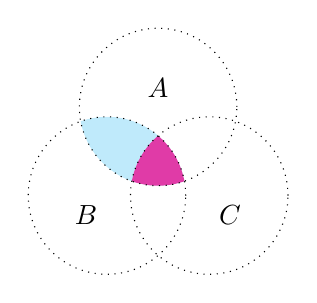
\begin{tikzpicture}
			\begin{scope}
				\clip \firstcircle;
				\fill[cyan,opacity=.25] \secondcircle;
			\end{scope}
			\begin{scope}
				\clip \firstcircle;
				\clip \secondcircle;
				\fill[magenta,opacity=.75] \thirdcircle;
			\end{scope}
			\draw[dotted] \firstcircle node[text=black,above] {$A$};
			\draw[dotted] \secondcircle node [text=black,below left] {$B$};
			\draw[dotted] \thirdcircle node [text=black,below right] {$C$};
		\end{tikzpicture}
		&&
		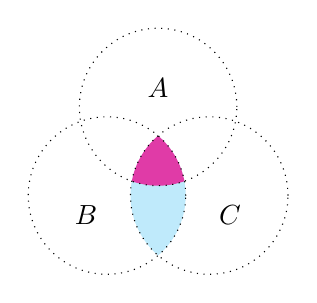
\begin{tikzpicture}
			\begin{scope}
				\clip \secondcircle;
				\fill[cyan,opacity=.25] \thirdcircle;
			\end{scope}
			\begin{scope}
				\clip \firstcircle;
				\clip \secondcircle;
				\fill[magenta,opacity=.75] \thirdcircle;
			\end{scope}
			\draw[dotted] \firstcircle node[text=black,above] {$A$};
			\draw[dotted] \secondcircle node [text=black,below left] {$B$};
			\draw[dotted] \thirdcircle node [text=black,below right] {$C$};
		\end{tikzpicture}
		\\
		(A \cap B) \cap C
		&=&
		A \cap (B \cap C)
	\end{array}\]

	\[\begin{array}{ccc}
		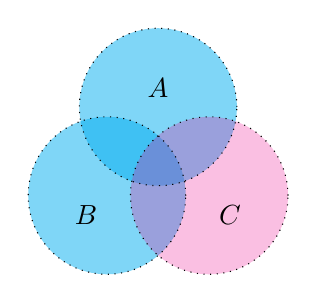
\begin{tikzpicture}
			\begin{scope}
				\fill[cyan,opacity=.5] \firstcircle;
				\fill[cyan,opacity=.5] \secondcircle;
			\end{scope}
			\begin{scope}
				\fill[magenta,opacity=.25] \thirdcircle;
			\end{scope}
			\draw[dotted] \firstcircle node[text=black,above] {$A$};
			\draw[dotted] \secondcircle node [text=black,below left] {$B$};
			\draw[dotted] \thirdcircle node [text=black,below right] {$C$};
		\end{tikzpicture}
		&&
		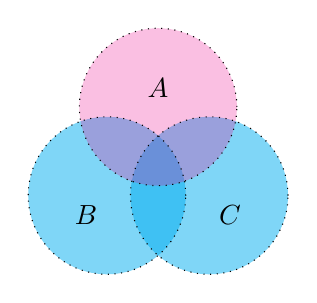
\begin{tikzpicture}
			\begin{scope}
				\fill[cyan,opacity=.5] \secondcircle;
				\fill[cyan,opacity=.5] \thirdcircle;
			\end{scope}
			\begin{scope}
				\fill[magenta,opacity=.25] \firstcircle;
			\end{scope}
			\draw[dotted] \firstcircle node[text=black,above] {$A$};
			\draw[dotted] \secondcircle node [text=black,below left] {$B$};
			\draw[dotted] \thirdcircle node [text=black,below right] {$C$};
		\end{tikzpicture}
		\\
		(A \cup B) \cup C
		&=&
		A \cup (B \cup C)
	\end{array}\]

	\[\begin{array}{ccc}
		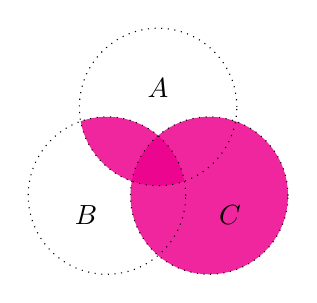
\begin{tikzpicture}
			\begin{scope}
				\clip \firstcircle;
				\fill[magenta,opacity=.85] \secondcircle;
			\end{scope}
			\begin{scope}
				\fill[magenta,opacity=.85] \thirdcircle;
			\end{scope}
			\draw[dotted] \firstcircle node[text=black,above] {$A$};
			\draw[dotted] \secondcircle node [text=black,below left] {$B$};
			\draw[dotted] \thirdcircle node [text=black,below right] {$C$};
		\end{tikzpicture}
		&&
		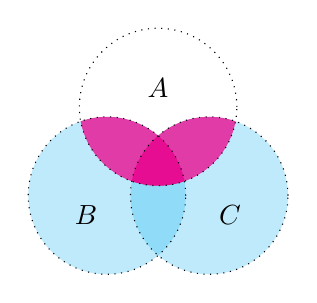
\begin{tikzpicture}
			\begin{scope}
				\fill[cyan,opacity=.25] \secondcircle;
				\fill[cyan,opacity=.25] \thirdcircle;
			\end{scope}
			\begin{scope}
				\clip \firstcircle;
				\fill[magenta,opacity=.75] \secondcircle;
				\fill[magenta,opacity=.75] \thirdcircle;
			\end{scope}
			\draw[dotted] \firstcircle node[text=black,above] {$A$};
			\draw[dotted] \secondcircle node [text=black,below left] {$B$};
			\draw[dotted] \thirdcircle node [text=black,below right] {$C$};
		\end{tikzpicture}
		\\
		(A \cap B) \cup C
		&\neq&
		A \cap (B \cup C)
	\end{array}\]

	\[\begin{array}{ccc}
		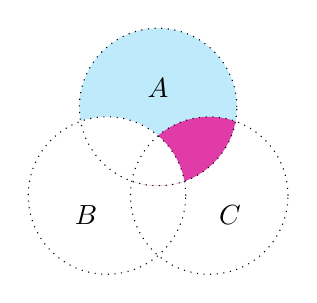
\begin{tikzpicture}
			\begin{scope}
				\fill[cyan,opacity=.25] \firstcircle;
				\clip \firstcircle;
				\fill[white] \secondcircle;
			\end{scope}
			\begin{scope}
				\clip \firstcircle;
				\fill[magenta,opacity=.75] \thirdcircle;
				\fill[white] \secondcircle;
			\end{scope}
			\draw[dotted] \firstcircle node[text=black,above] {$A$};
			\draw[dotted] \secondcircle node [text=black,below left] {$B$};
			\draw[dotted] \thirdcircle node [text=black,below right] {$C$};
		\end{tikzpicture}
		&&
		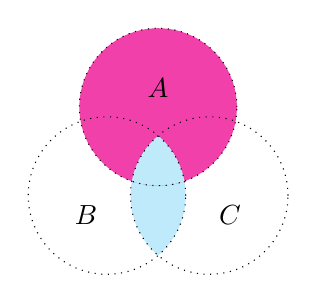
\begin{tikzpicture}
			\begin{scope}
				\fill[magenta,opacity=.75] \firstcircle;
				\clip \secondcircle;
			\end{scope}
			\begin{scope}
				\clip \firstcircle;
				\clip \secondcircle;
				\fill[white] \thirdcircle;
			\end{scope}
			\begin{scope}
				\clip \secondcircle;
				\fill[cyan,opacity=.25] \thirdcircle;
			\end{scope}
			\draw[dotted] \firstcircle node[text=black,above] {$A$};
			\draw[dotted] \secondcircle node [text=black,below left] {$B$};
			\draw[dotted] \thirdcircle node [text=black,below right] {$C$};
		\end{tikzpicture}
		\\
		(A - B) \cap C
		&\neq&
		A - (B \cap C)
	\end{array}\]
\end{itemize}

\section*{Problem 4}

\begin{itemize}
\item
  Let \emph{J} abbreviate \emph{John comes}. Let \emph{B} abbreviate
  \emph{Bill comes}. Let \emph{S} abbreviate \emph{the party will be a
  success}.
\item
  The speaker said \emph{if J and B then S}. Call this utterance $p$.
\item
  The speaker did \textbf{not} say \emph{if J or B then S}. Call this would-be
  utterance $p^+$.
\item
  $p^+$ is stronger than $p$: from \emph{if J or B then S} you can
  conclude \emph{if J and B then S}. (In class it was debated whether this holds
  \emph{in the general case}, but it clearly holds here. Notice that this
  \emph{or} is to be interpreted \textbf{inclusively}, i.e.~as \emph{at least
  one of J, B}.)
\item
  Therefore (assuming $p^+$ was Relevant), Quantity and
  Quality force us to conclude the speaker does not believe $p^+$.
  (Otherwise, the speaker should have said $p^+$!)
\item
  Therefore (assuming the speaker is an authority, i.e.~opinionated and
  knowledgeable) we conclude that $p^+$ is false. That is, we conclude that
  it's false that John or Bill coming guarantees a successful party. Call this
  inference $p^-$. This is as far as I was expecting anyone to get in the
  homework. Feel free to stop reading here.
\item
  Still with me? Ok. A question asked in class was: from the speaker's
  original utterance of $p$, we actually seem to conclude something that
  seems strictly \textbf{stronger} than $p^-$, namely that if just one of them
  comes, the party won't be a success.
\item
  Here, we'll chalk this up to something called \textbf{Conditional Excluded
  Middle} (CEM essentially says that for any $p$ and $q$, either $p$ guarantees
  $q$, or $p$ guarantees $\emph{not }q$). We reason as follows:
  	\[
	\begin{array}{l@{}lc}
		&\text{John and Bill both coming guarantees success.} & (p)
		\\
		&\text{At least one coming doesn't guarantee success.} & (p^-)
		\\\hline
		\therefore~&\text{Only John or only Bill coming doesn't guarantee success.} & (p^{\star})%
	\end{array}
	\]
\noindent Together with CEM, $p^{\star}$ entails that only John or only Bill coming guarantees a \textbf{lack of success}.\footnote{There is an interesting issue that comes up here: if we applied CEM to $p^-$, we'd derive something inconsistent with $p$ (i.e.~at least one coming guarantees a lack of success). Why do we actually apply it to $p^{\star}$? This actually has an answer in the modern literature on scalar implicature. I can give some pointers if folks are interested.}%
\item
  If you'd like to read more about reverse implicatures, I have some
  older notes from another class that I've uploaded to the course
  website. Feel free to peruse, or not.
\end{itemize}


\end{document}
